% Yutong Xue's hardware field-notebook report style.
\documentclass[lang=en,11pt,a4paper,bibend=bibtex]{elegantpaper}
\usepackage{xeCJK}
\setCJKmainfont{FandolSong-Regular.otf}
\setCJKsansfont{FandolSong-Regular.otf}
\setCJKmonofont{FandolSong-Regular.otf}
\usepackage{tikz,pgfplots,tabularx,titlesec,fancyhdr}
\usetikzlibrary{arrows.meta,positioning,calc}
\pgfplotsset{compat=1.18}
\geometry{left=23mm,right=23mm,top=21mm,bottom=22mm,headheight=15pt,headsep=7mm}
\linespread{1.10}
\setlength{\parindent}{0pt}
\setlength{\parskip}{5pt}
\setlength{\emergencystretch}{2em}
\definecolor{accent}{HTML}{234D64}
\definecolor{muted}{HTML}{59646C}
\definecolor{light}{HTML}{F0F4F6}
\hypersetup{colorlinks=true,linkcolor=accent,urlcolor=accent}
\titleformat{\section}{\Large\sffamily\bfseries\color{accent}}{\thesection}{0.6em}{}
\titleformat{\subsection}{\normalsize\sffamily\bfseries}{\thesubsection}{0.6em}{}
\titlespacing*{\section}{0pt}{9pt}{8pt}
\titlespacing*{\subsection}{0pt}{8pt}{3pt}
\pagestyle{fancy}
\fancyhf{}
\fancyhead[L]{\small\sffamily\color{muted}EXPERIMENT 2\enspace /\enspace ROBOMASTER EP}
\fancyhead[R]{\small\sffamily\color{muted}\studentname}
\fancyfoot[L]{\small\sffamily\color{muted}\studentid\quad\textbullet\quad Individual laboratory report}
\fancyfoot[R]{\small\sffamily\thepage}
\renewcommand{\headrulewidth}{0.3pt}
\renewcommand{\footrulewidth}{0pt}
\captionsetup{font=small,labelfont=bf,labelsep=period,skip=5pt,hypcap=false}
\renewcommand{\arraystretch}{1.18}
\newcolumntype{Y}{>{\raggedright\arraybackslash}X}
\newcommand{\code}[1]{{\small\nolinkurl{#1}}}
\newcommand{\source}[1]{{\small\color{muted}Source: #1}\par}
\newcommand{\reportnote}[1]{\par\smallskip\noindent\colorbox{light}{\parbox{\dimexpr\linewidth-2\fboxsep}{\small #1}}\par\smallskip}
\newcommand{\reporttitle}[1]{\vspace*{2mm}{\small\sffamily\bfseries\color{accent}FIXED-POINT PICK-AND-PLACE}\par\vspace{2mm}{\LARGE\sffamily\bfseries #1\par}\vspace{3mm}{\large\studentname\enspace\studentcn}\par{\small Student ID: \studentid\quad |\quad Individual report}\par\vspace{3mm}\hrule\vspace{3mm}}
\tikzset{box/.style={draw=accent,fill=light,rounded corners=2pt,align=center,font=\small,minimum height=9mm},arr/.style={-{Latex[length=2mm]},thick,draw=accent}}
\newcommand{\teamtable}{%
\par\smallskip
\begingroup\small\renewcommand{\arraystretch}{1.08}
\begin{tabularx}{\linewidth}{@{}>{\raggedright\arraybackslash}p{25mm}>{\raggedright\arraybackslash}p{21mm}Y@{}}\toprule
Member & Work area & Main responsibility \\\midrule
Ning Bo & Simulation & Set up the environment and scene; load models and launch the simulation.\\
Huang Junbiao & Simulation & Work on the motion program and debug grasping, transfer and repeated cycles.\\
Qi Yongyue & Simulation results & Organize logs, analyse results and prepare report material.\\
Bao Lintai & Hardware & SDK communication, task sequence, chassis turn/return and exception handling; joint trials.\\
Xue Yutong & Hardware & Pick/release waypoints, approach/lift heights, gripper adjustment and retention checks; joint trials.\\\bottomrule
\end{tabularx}\par\endgroup}
\newcommand{\commonrequirements}{%
\section{Experiment requirements and individual scope}
The experiment develops a fixed-point grasping task without visual localization: home, approach A, descend, grip, lift, transfer to B, release and return. The course requires a complete simulation launch, state publication, saved trajectories/results/errors, joint and reachability checks, and at least four successful transfers in five consecutive trials. Hardware verification additionally requires supervised low-speed operation, safe failure handling and individual safety-operation checks [1].

Because of equipment availability, our group used the DJI RoboMaster EP arm and gripper instead of the specified mechArm 270. The simulation uses ROS 2 Humble, Gazebo Fortress and custom kinematics/control on a Jetson Linux system. The physical implementation uses the RoboMaster Python SDK. This is a platform adaptation, not an unchanged ROS 2 hardware backend.
}
\newcommand{\commonlimits}{%
\reportnote{Scope of evidence. Simulation repeats A$\rightarrow$B and verifies home after every cycle; the object is reset only between cycles. Hardware alternates A/B, pauses for human grasp confirmation and returns home after all five cycles. Shared ROS 2 interfaces, parameter-only hardware switching and each member's safety check are not demonstrated by the supplied records.}}
\newcommand{\mainresults}{%
\begin{center}\small
\begin{tabular}{@{}crrrcc@{}}\toprule
Cycle & Error (mm) & Heading ($^\circ$) & Time (s) & Placed & Home \\\midrule
1 & 2.274 & 0.445 & 67.01 & Yes & Yes\\
2 & 5.604 & 0.329 & 59.72 & Yes & Yes\\
3 & 4.192 & 0.404 & 60.92 & Yes & Yes\\
4 & 4.577 & 0.459 & 61.09 & Yes & Yes\\
5 & 5.144 & 0.405 & 61.29 & Yes & Yes\\\bottomrule
\end{tabular}
\end{center}
\source{Recorded simulation run \code{20260913_153855_682865/results.json}; error is horizontal distance from configured B, heading is absolute home-heading error.}}
\newcommand{\hardwareresult}{%
\subsection{Physical validation: team-observed outcome}
The team confirmed that all five hardware transfers succeeded with no observed abnormalities. Cycles 1, 3 and 5 moved A$\rightarrow$B; cycles 2 and 4 moved B$\rightarrow$A. Each lift was followed by a fresh human \code{y} confirmation before rotation; final heading restoration and homing followed cycle 5. This is an observed 5/5 result, not an instrumented precision or timing measurement. No real-hardware position-error, duration or force data are available, and five successes do not establish long-run reliability.}
\newcommand{\githubsection}{%
\clearpage
\section{Shared GitHub repository and commit evidence}
The complete group archive is stored in the
\href{https://github.com/ccx8kg5qpd-debug/robomaster-ep-fixed-point-grasping}
{shared public GitHub repository}. The repository address is
\nolinkurl{github.com/ccx8kg5qpd-debug/robomaster-ep-fixed-point-grasping}.
It contains the simulation and hardware programs, model resources, saved results,
the complete simulation recording and all five individual report sources.

\begin{center}
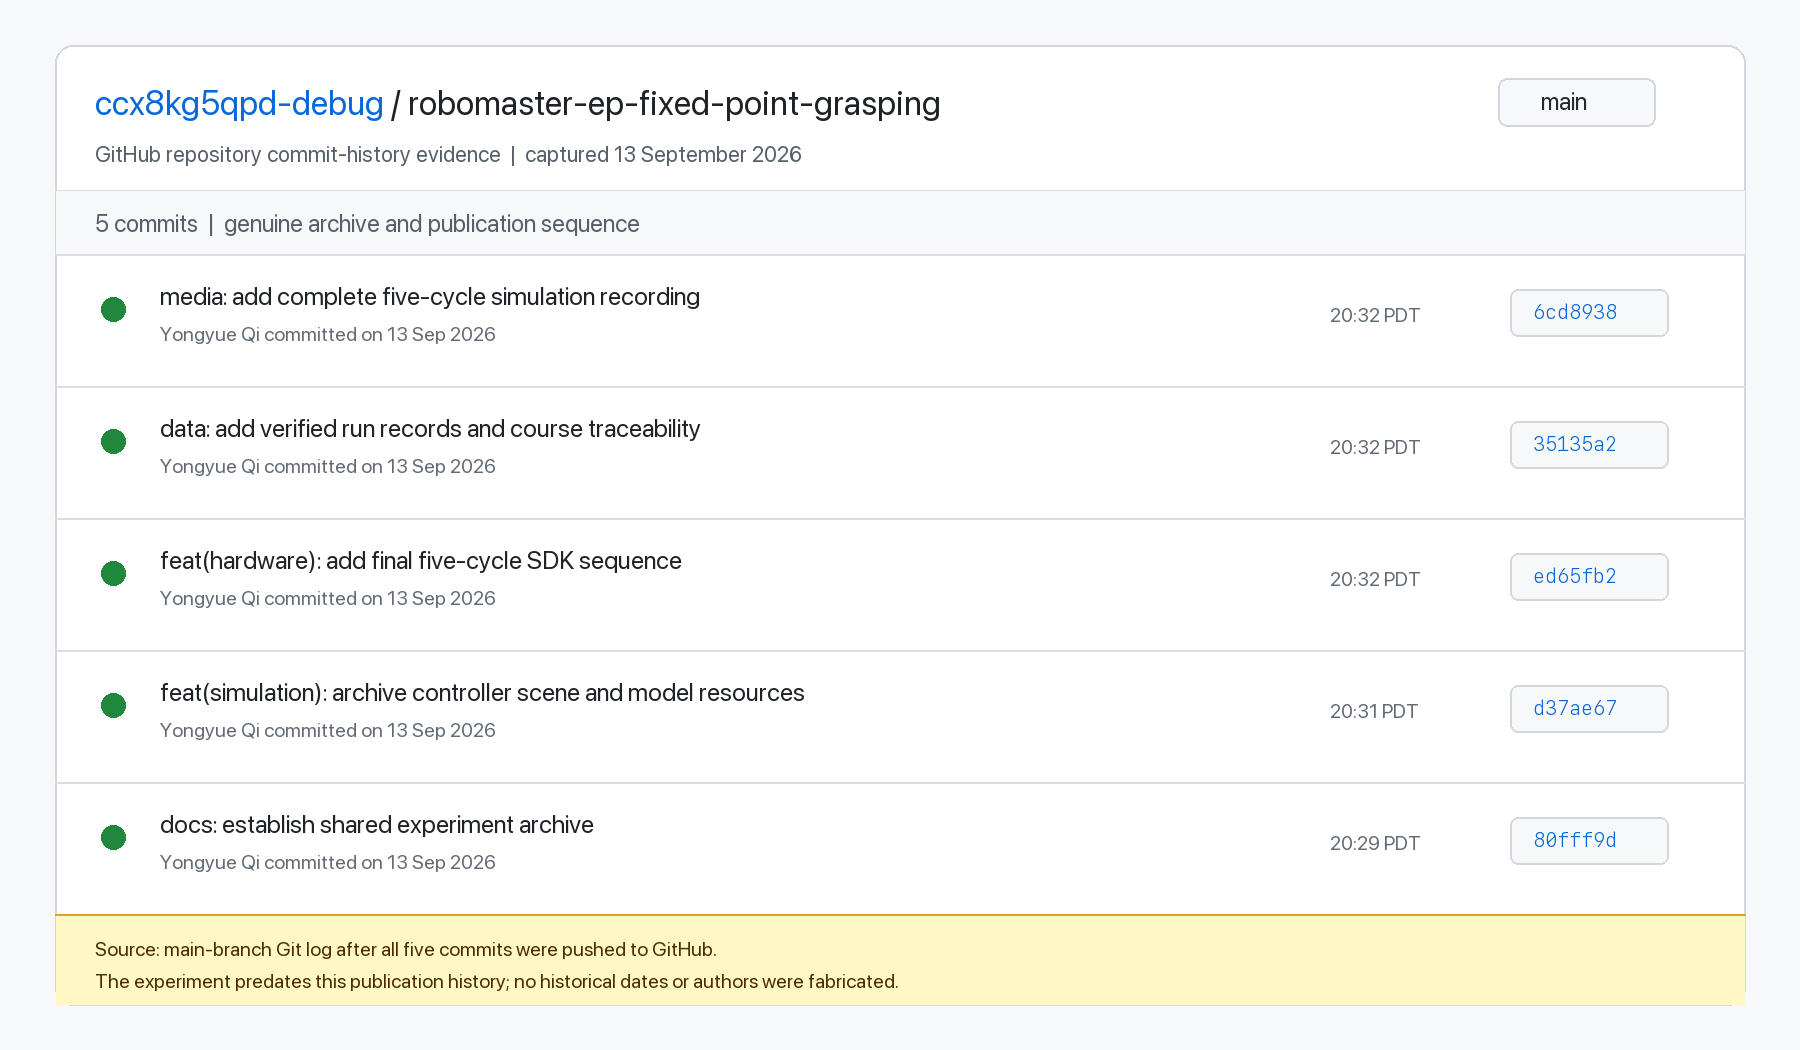
\includegraphics[width=\linewidth]{assets/commit_history_snapshot.png}
\captionof{figure}{Commit-history evidence captured after the first five project
materials commits had been pushed to the shared GitHub repository.}
\end{center}

\reportnote{Traceability note. The experiment was completed before the GitHub
repository was assembled. These genuine commits document the later review,
organization and publication sequence; they are not presented as a fabricated
contemporaneous development history. The screenshot records the five commits
visible at capture time, before this revised report was added.}
}
\newcommand{\referencesblock}{%
\section*{Sources and traceability}
{\footnotesize
[1] Course handout, \emph{Fixed-Point Robotic-Arm Grasping: Simulation Development and Hardware Validation}, S16--S20 / E5; individual-report assignment requirements.\par
[2] Shared team repository, \href{https://github.com/ccx8kg5qpd-debug/robomaster-ep-fixed-point-grasping}{robomaster-ep-fixed-point-grasping}, assembled 13 September 2026: simulation source/configuration, \code{real_v2_five_cycles_manual.py}, saved logs and reports. Primary numerical record: \code{20260913_153855_682865}.\par
[3] Team conversation fact-check materials, 13 September 2026, for development history; subsequent team confirmation for the completed five-cycle hardware run. Historical failures are not counted as final-run failures.\par
[4] Community model resources: \href{https://github.com/jeguzzi/robomaster_ros}{jeguzzi/robomaster\_ros}, archived commit \code{c05a39d7f0fa}. Report layout uses \href{https://ctan.org/pkg/elegantpaper}{ElegantPaper}, distributed under LPPL 1.3c.
}}

\definecolor{accent}{HTML}{286043}
\definecolor{muted}{HTML}{5F685E}
\definecolor{light}{HTML}{F1F5E9}
\definecolor{fieldtan}{HTML}{D7BE8A}
\geometry{left=27mm,right=20mm,top=21mm,bottom=22mm,headheight=16pt,headsep=7mm}
\hypersetup{linkcolor=accent,urlcolor=accent}
\titleformat{\section}{\Large\sffamily\bfseries\color{accent}}{\fcolorbox{accent}{light}{\thesection}}{0.75em}{}
\titleformat{\subsection}{\normalsize\sffamily\bfseries\color{accent}}{\thesubsection}{0.55em}{}
\fancyhead[L]{\small\sffamily\bfseries\color{accent}HARDWARE FIELD NOTE / E2}
\fancyhead[R]{\small\sffamily\color{muted}\studentname}
\fancyfoot[L]{\scriptsize\sffamily\color{muted}Waypoint and gripper verification record}
\fancyfoot[R]{\small\sffamily\bfseries\color{accent}\thepage}
\renewcommand{\headrulewidth}{0.8pt}
\renewcommand{\reportnote}[1]{\par\smallskip\noindent\colorbox{light}{\parbox{\dimexpr\linewidth-2\fboxsep}{\small\textcolor{accent}{\textbf{FIELD CHECK}}\quad #1}}\par\smallskip}
\renewcommand{\reporttitle}[1]{\vspace*{2mm}{\small\sffamily\bfseries\color{accent}FIELD NOTE 02 / PHYSICAL SYSTEM}\par\vspace{3mm}{\color{fieldtan}\rule{\linewidth}{3pt}}\par\vspace{5mm}{\fontsize{22}{27}\selectfont\sffamily\bfseries #1\par}\vspace{4mm}{\large\sffamily\studentname\enspace\studentcn\par}{\small Student ID: \studentid\quad|\quad Individual hardware notebook}\par\vspace{4mm}}

\newcommand{\studentname}{Xue Yutong}
\newcommand{\studentcn}{薛羽桐}
\newcommand{\studentid}{24020036072}
\begin{document}
\reporttitle{Hardware Waypoint\\Adjustment and Gripper Testing}
\commonrequirements
\subsection{My responsibility in the hardware pair}
Bao Lintai and I share the hardware and physical experiment. My main scope is the pick/release positions, approach and lift heights, gripper opening/closing and object retention. Bao's main scope is SDK communication, program sequencing, chassis turning, return motion and exception handling. We share physical setup, integrated testing and reviewing the five transfers, with complementary attention to the arm settings and the complete motion sequence. Ning Bo and Huang Junbiao handle simulation setup and programming, while Qi Yongyue organizes the results and report material.
\teamtable
\commonlimits
\section{Physical setup and waypoint adjustment}
\subsection{What fixed-point operation assumes}
No vision system locates the cube in this experiment. A usable grasp therefore requires agreement between the physical source position and the commanded gripper position. The cube, robot starting pose and placement region must be arranged consistently. The working area must also accommodate the chassis turn and the arm's sweep, not just the two endpoints.

My hardware scope connects these physical conditions to the arm parameters. A failed pickup should first be separated into a position problem, a height problem or a grip-retention problem. Increasing the closing command cannot correct a cube that lies outside the fingertip region. Similarly, changing the base turn does not fix an incorrect descent height.
\begin{center}
\begin{tabular}{@{}lrrl@{}}\toprule
Final SDK waypoint & $x$ (mm) & $y$ (mm) & Tuning concern\\\midrule
HOME & 82 & 80 & Retracted return position\\
HIGH & 191 & 80 & Extension at the high level\\
HOVER & 191 & $-1$ & Approach and lifted-object position\\
GRASP & 191 & $-51$ & Pick and release level\\\bottomrule
\end{tabular}
\end{center}
\source{Final hardware script. These are the saved settings, not a newly measured calibration dataset.}
\subsection{Reasoning about the vertical motion}
The second SDK arm coordinate is the vertical coordinate used by the script. HOVER and GRASP have the same $x$, and their vertical difference is
\begin{equation}
\Delta y=(-1)-(-51)=50\ \mathrm{mm}.
\end{equation}
This gives the commanded lift used to check retention before turning. It does not establish an independently measured 50 mm object displacement or a universal safe clearance above every surface.

Initial motion passes through HOME, HIGH and HOVER before descent. The high-level extension separates reaching outward from moving down toward the cube. In reviewing the settings, the important checks are fingertip alignment at the low point and sufficient object clearance at the lifted point. Adjustments require a stopped, controlled test procedure; the report does not invent intermediate trial coordinates that were not recorded.
\subsection{Coordinate systems must remain distinct}
The SDK uses millimetre pairs with its own reference. Simulation uses model/world coordinates in metres, including a 0.060 m vertical model offset. Multiplying a simulation coordinate by 1,000 is not a complete physical calibration. The saved hardware waypoints must be treated as device-specific settings and checked against the real arrangement.
\clearpage
\section{Gripper adjustment and retained-object verification}
\subsection{Opening, closing and dwell}
The final script opens with SDK power setting 30, waits 1.5 s and pauses the gripper. It closes with power setting 100, waits 3 s and pauses again. These settings and dwell times form part of the hardware grasp procedure; they are not force measurements. A command being accepted does not itself prove that the cube is held.

My part of the hardware work covers the relation between these commands and the object: whether the opening permits approach, whether the low point aligns the fingertips with the cube, and whether retention survives lifting. Bao's sequence must wait for these operations in the correct order. Both parts need to be checked together before treating the complete transfer as ready.
\begin{center}\small
\begin{tabularx}{\linewidth}{@{}p{31mm}YY@{}}\toprule
Check point & Physical question & Associated parameter or decision\\\midrule
Before descent & Is the source aligned and the gripper open? & Source arrangement; HOVER; opening command.\\
At the low point & Do the fingers engage the object region? & GRASP coordinates and object position.\\
After closure & Does the cube rise with the fingers? & Closing command, dwell and 50 mm lift.\\
Before rotation & Is retention clearly confirmed? & Fresh human confirmation; otherwise no transfer.\\
After release & Does the object remain at the destination? & Release level, opening dwell and retreat.\\\bottomrule
\end{tabularx}
\end{center}
\subsection{Why confirmation follows the lift}
An earlier, abandoned checking script reported a closed gripper but no object. This illustrates why closure is not equivalent to retention. The final manual script instead lifts to HOVER, stops the chassis, clears pending terminal input and waits up to 30 s for a fresh \code{y}. The decision is based on the current lifted object, not an earlier key press.

If confirmation is absent, no transfer turn or automatic homing is commanded; the script stops above the source and performs cleanup. This limits additional motion with an uncertain grasp. The operator and observer must communicate clearly, and object adjustment must not be attempted by hand while the task can resume.
\subsection{Two people jointly test the mechanism}
The hardware pair shares integrated trials rather than dividing the experiment into one permanent operator and one passive helper. During an individual run, one person handles controls and the other watches the moving mechanism; both need to understand the waypoint and retention checks. This defines how the responsibilities cooperate, not a claim of separately documented individual safety qualifications.
\clearpage
\section{Integration with turning and repeated transfers}
\subsection{Arm settings affect the base transfer}
The object must be retained at HOVER before the chassis turns. The script commands $+32^\circ$ on odd cycles and $-32^\circ$ on even cycles at $12^\circ$/s. Bao's turn/return logic and my arm/gripper settings therefore meet at a specific condition: a confirmed, lifted object. A correct base command cannot compensate for a slipping grasp, while a retained object cannot compensate for an incorrect destination alignment.

The script lowers to GRASP, opens, waits and retreats to HOVER at the destination. Hardware then reverses direction for the next cycle, leaving the released object as the next source. It does not require manual replenishment at A after every success. After five cycles, heading is restored and the arm returns through HIGH to HOME.
\begin{center}
\begin{tabular}{@{}clll@{}}\toprule
Cycle & Direction & Team-confirmed result & Abnormality\\\midrule
1 & A$\rightarrow$B & Successful & None observed\\
2 & B$\rightarrow$A & Successful & None observed\\
3 & A$\rightarrow$B & Successful & None observed\\
4 & B$\rightarrow$A & Successful & None observed\\
5 & A$\rightarrow$B & Successful & None observed\\\bottomrule
\end{tabular}
\end{center}
\source{Team confirmation of the final five-cycle hardware workflow and outcome. No separate personal measurement log is claimed.}
\subsection{Results and what they establish}
The observed hardware result was 5/5 successful transfers with no abnormalities, meeting the at-least-4/5 transfer criterion for this sample. It supports the combined use of the final waypoints, gripper sequence and base motion. It does not identify the effect of one parameter in isolation: there is no recorded controlled comparison of alternative heights or dwell times.

The recording-associated simulation also achieved 5/5, with mean horizontal placement error 4.358 mm and maximum 5.604 mm. Those are simulation measurements, not physical calibration errors. Hardware error, duration and force measurements were not supplied. The simulated cube's 50 g mass is likewise a model parameter, not a recorded weighing of the real object.
\subsection{Difference from the simulated test}
Simulation repeats A$\rightarrow$B, checks contact/height feedback and resets the cube only after per-cycle homing. Hardware alternates directions, uses human retention confirmation and completes its final return after cycle 5. The physical setup and parameter review must follow this hardware sequence. The direct SDK script also differs from the handout's shared-ROS-interface objective.
\clearpage
\section{Problems, solutions and individual reflection}
\subsection{Distinguishing misalignment from weak retention}
A gripper can close around empty space because of source-position error, or engage the cube and then lose it during lifting. These require different investigations. I would check source/fingertip alignment and the low waypoint before changing grip settings; after engagement is confirmed, I would examine closure, dwell and lift retention. This avoids attributing every failure to insufficient closing power. The report uses the archived final settings without inventing a parameter-search history.
\subsection{Selecting useful approach and lift heights}
A low approach risks unwanted contact, while changing a height without considering the robot reference can produce an unintended movement. The final HOME--HIGH--HOVER--GRASP arrangement separates extension, approach and descent. My interpretation is to review each segment in the actual working area, then confirm clearance with the retained object, not just an empty gripper. The numerical 50 mm lift is a command difference, not proof of every safety margin.
\subsection{Release quality affects the next pickup}
Because hardware reverses direction, an object left poorly aligned after release can become the next pickup problem. Release level, opening time and retreat should therefore be reviewed alongside grasping, rather than treating the trial as finished the instant the gripper opens. The five successes show that the final combined sequence worked in the confirmed run, but do not provide a measured placement-tolerance study.
\subsection{Shared testing, distinct technical focus}
My contribution is centred on the physical arm--object interaction and its waypoint/gripper settings; Bao's is centred on communication and whole-program sequencing. Joint trials are where we check their compatibility. This division gives both hardware members a substantive tuning and testing role instead of assigning all technical work to one person.

A useful follow-up would record the waypoint version, closure settings, observed lift retention and release position for each trial. Changing one factor at a time would make the effect of a change clearer. No additional fault tests, force measurements or safety qualifications are claimed here. My conclusion is that successful fixed-point grasping depends on coordinated setup, positioning and retention checks, not a closed-gripper indication alone.
\githubsection
\referencesblock
\end{document}
